\documentclass{standalone}
\usepackage{amsmath}
\usepackage[dvipsnames]{xcolor}
\usepackage{tikz} 
\usetikzlibrary{arrows, decorations.markings,decorations.pathreplacing,angles,quotes}
\usepackage{microtype}
\usepackage{fourier}

\definecolor{nblue}{RGB}{31, 119, 180}

\begin{document}

\begin{tikzpicture}
   		\node[anchor=south west,inner sep=0] (Bild) at (0,0) {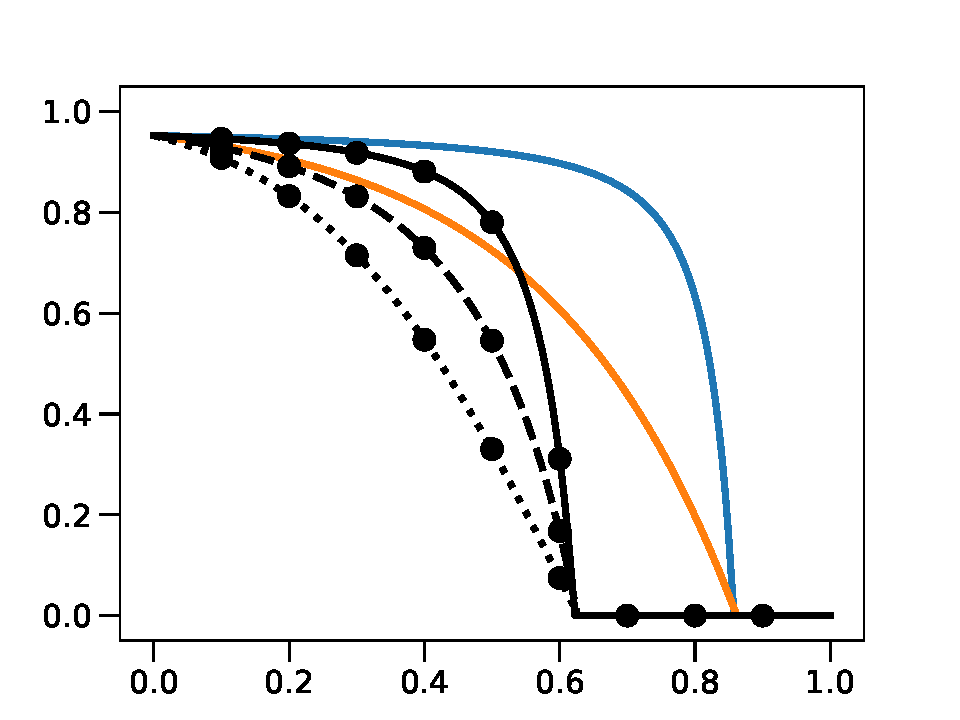
\includegraphics[scale=0.39]{figS2b_blank.pdf}};
   		\begin{scope}[x=(Bild.south east),y=(Bild.north west)]
					  	
        	\draw (.5,-0.035) node {antiviral drug efficacy $\varepsilon_j$};
        	\draw (0.0,0.5) node [rotate=90] {est. probability $\psi_j$};
        	 
        	        	        	
        	\end{scope}
\end{tikzpicture}

\end{document}